\section{Formal Analysis Using Alloy}
Alloy is a specification language for describing, designing, and verifying the behavior of complex systems.
The language is based on first-order logic, and has a mathematical foundation that allows for automated reasoning
about the correctness of designs.
Once a model has been defined, it will be analyzed using a tool that supports Alloy, such as AlloyAnalyzer. This tool can automatically check
whether the model satisfies the specified constraints and properties, and can also be used to explore the space of
possible behaviors to find designs that meet the desired criteria.

\subsection{Objectives of the analysis}
The main goal of the formal analysis is to formally describe the domain and properties of the system to be.

\subsubsection{Reservation Model}
The reservation of a CP is a core part of the System to Be.
The Alloy model for verifying reservations of charging points includes abstractions
for the entities involved in a reservation, such as charging points, charging sockets and reservation times.
It also includes constraints on the relationships between these entities, such as the fact that a charging socket
can be reserved by one vehicle at a time, or that a vehicle can be charged by one charging socket at a time.

\lstinputlisting[language=C, basicstyle=\ttfamily\footnotesize]{src/alloy/reservationModel.als}
\begin{figure}[H]
    \centering
    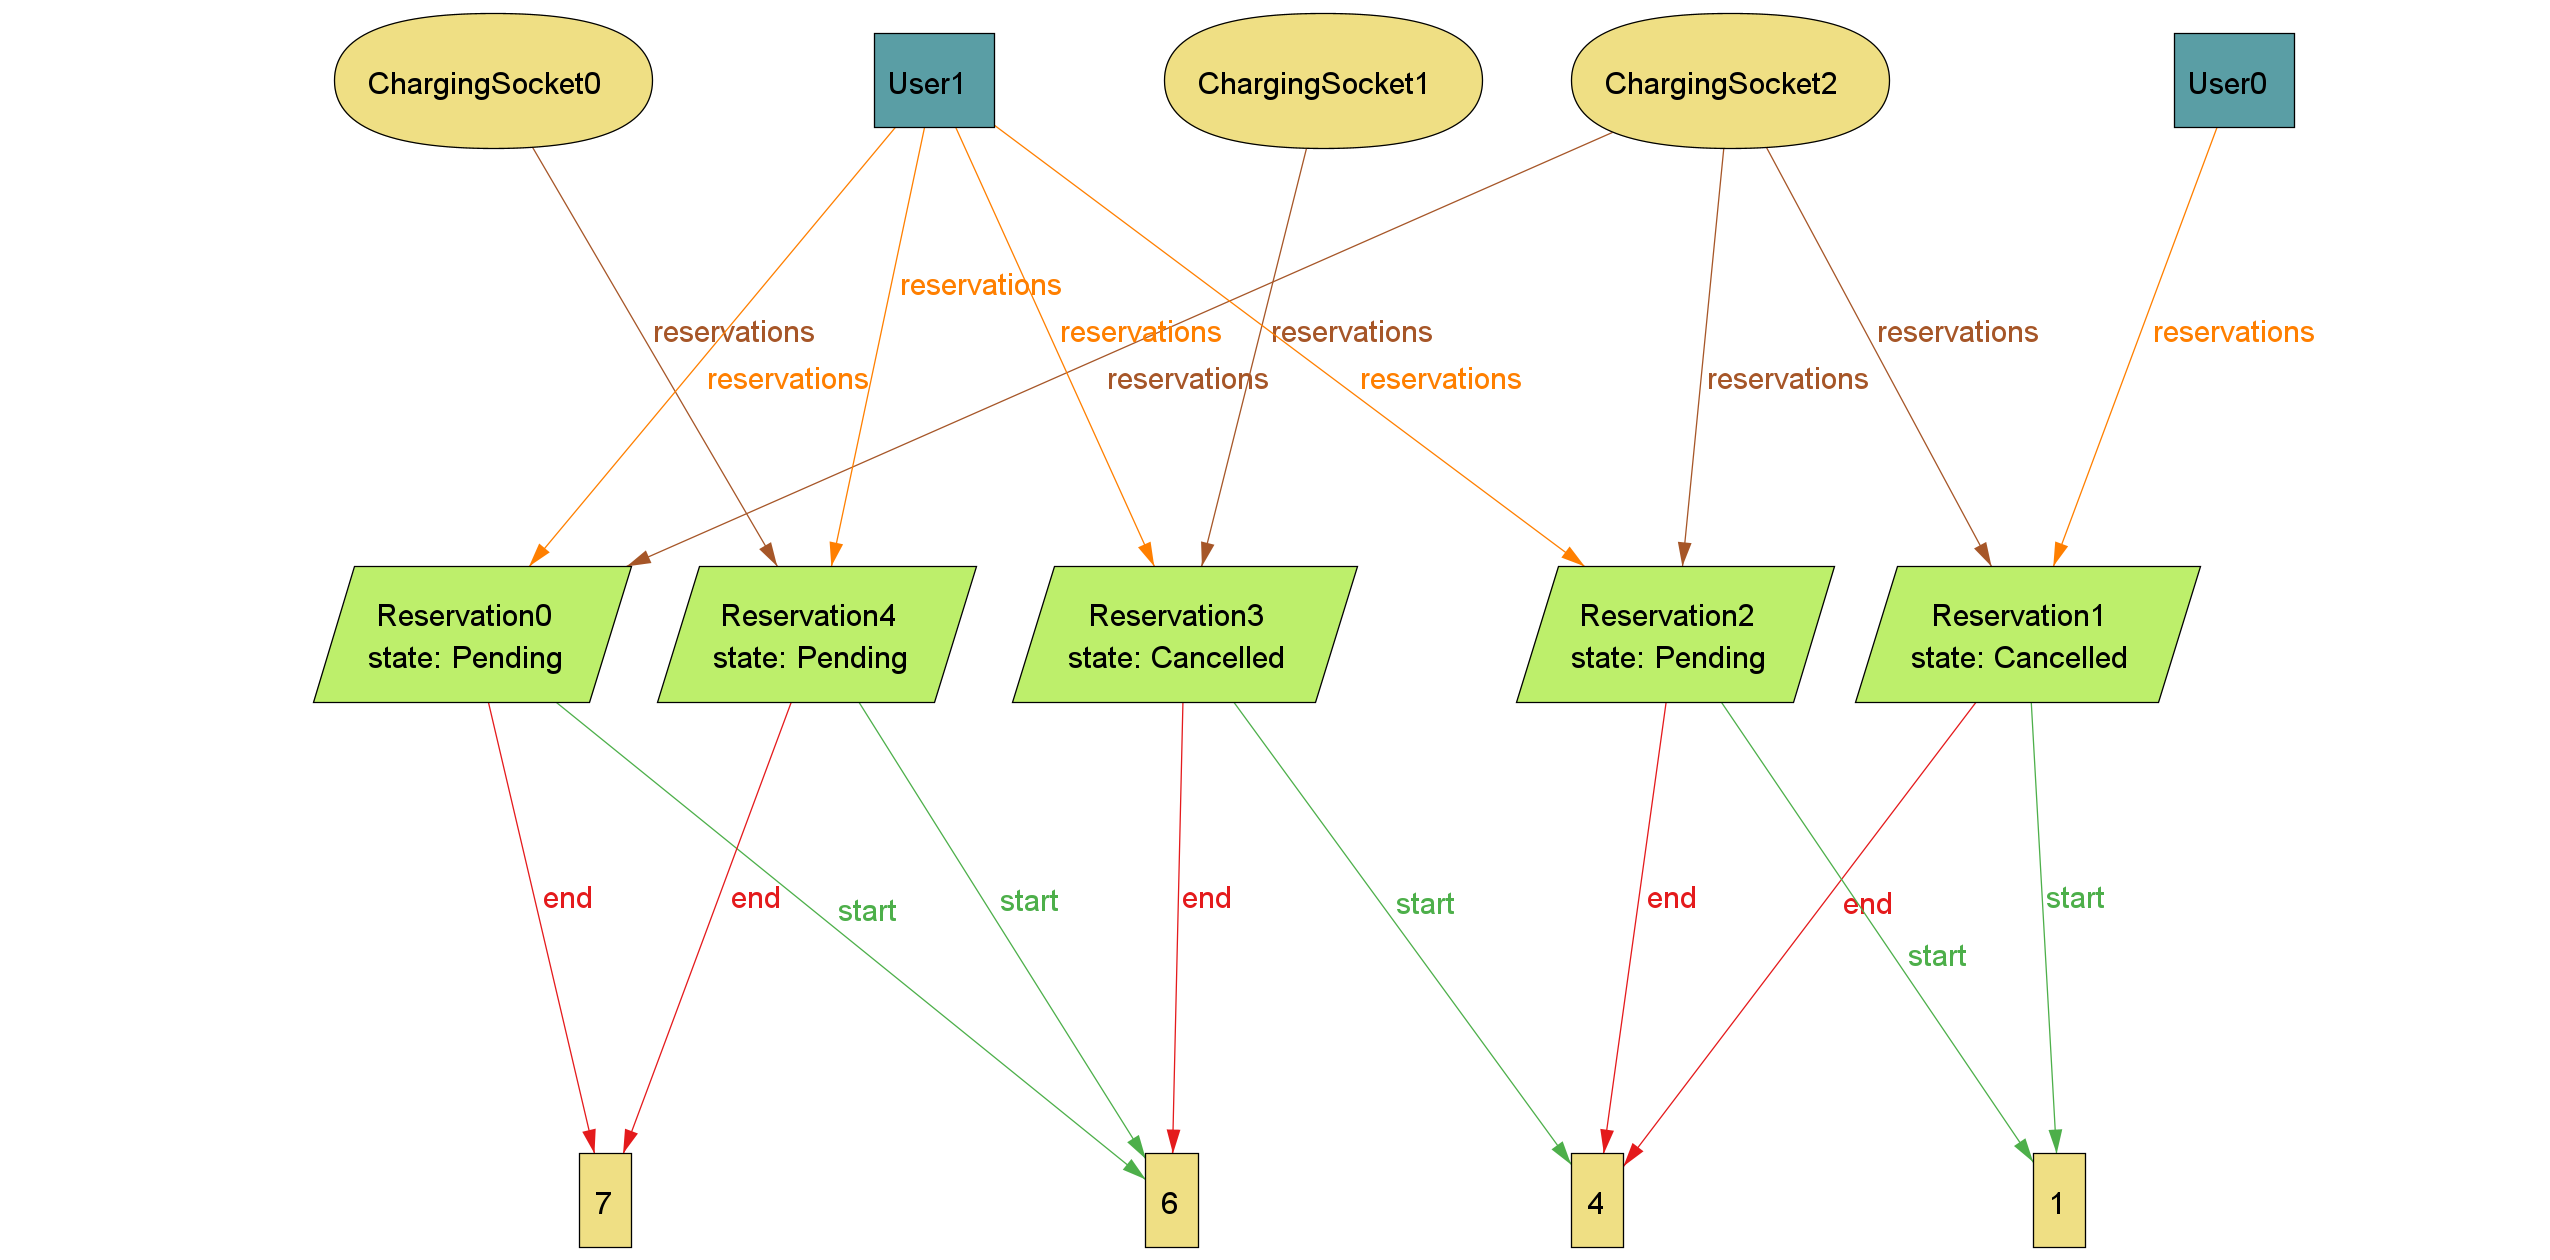
\includegraphics[width=1\textwidth]{src/alloy/reservationModel.png}
\end{figure}
\begin{figure}[H]
    \centering
    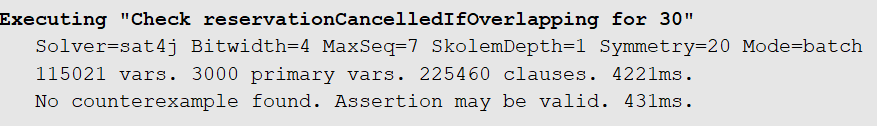
\includegraphics[width=1\textwidth]{src/alloy/reservationModel_assertion.png}
\end{figure}
